% ------------------------------------------ INTRODUCTIONS ------------------------------------------ %
\subsection{Tools Introduction: GDB}
\subsubsection*{Problem Domain}
This lab covers the following aspects of the reverse engineering problem domain created by us: \\
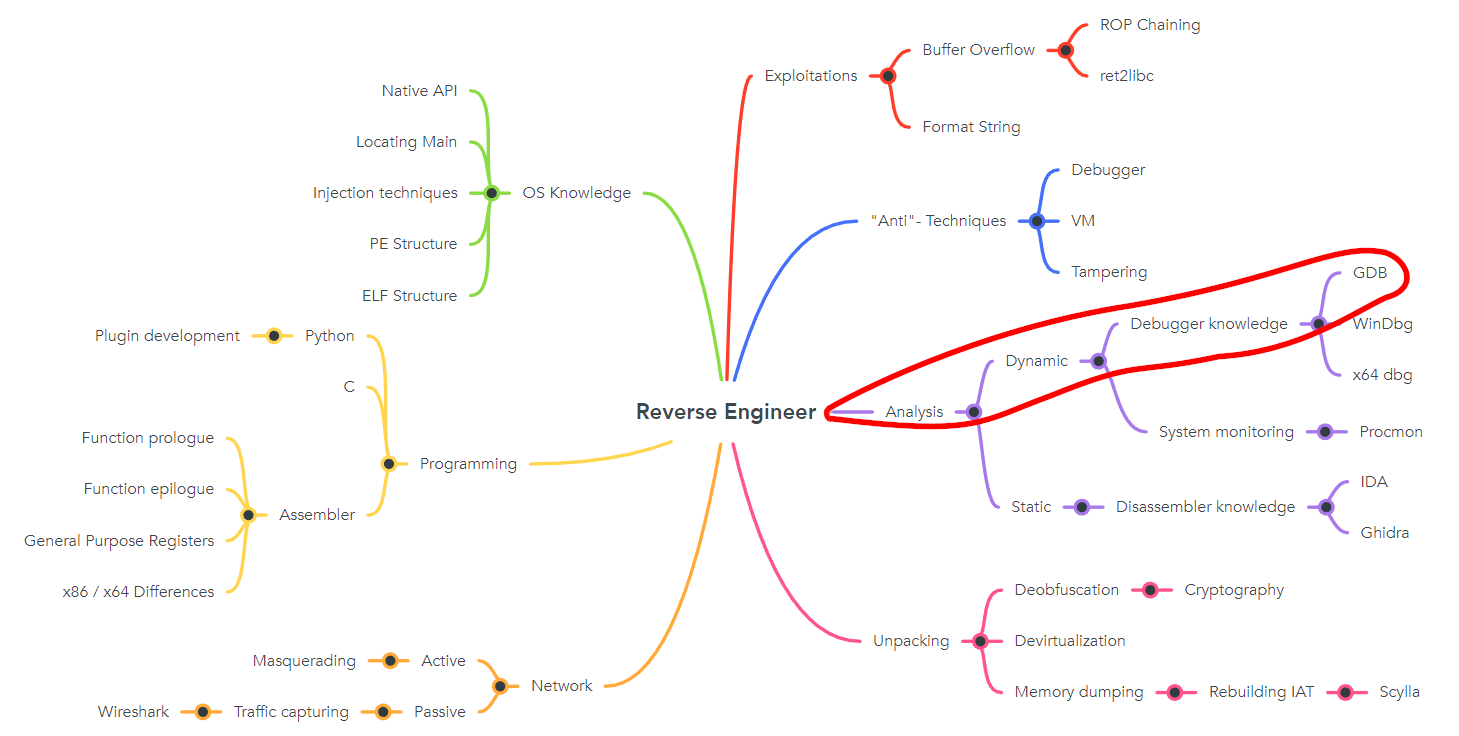
\includegraphics[width=\textwidth]{resources/GDBIntro-overview-light.png}
\subsubsection*{Content}
This introduction is used to explain the basic functionalities of the tool used in some of the labs. In this case GDB (GNU Debugger).
\subsubsection*{Choice of Topic}
The solutions and tips in the labs are given via screenshots or explanations. If a student wants to use a different tool he / she is free to do so. It is important that the tools used in the example solutions are known to the students. This makes it easier for them to understand each step and, if they are stuck at any point, follow the intructions on how to solve it. 
\subsubsection*{Objectives}
\begin{itemize}
    \item Learn about GDB and how to use the different commands available
\end{itemize}
\subsubsection*{Grading}
The labs are not graded since they are only used as a lookup. They have a flag to make sure the students have read the tools.
\pagebreak

\subsection{Tools Introduction: x64dbg}
\subsubsection*{Problem Domain}
This lab covers the following aspects of the reverse engineering problem domain created by us: \\
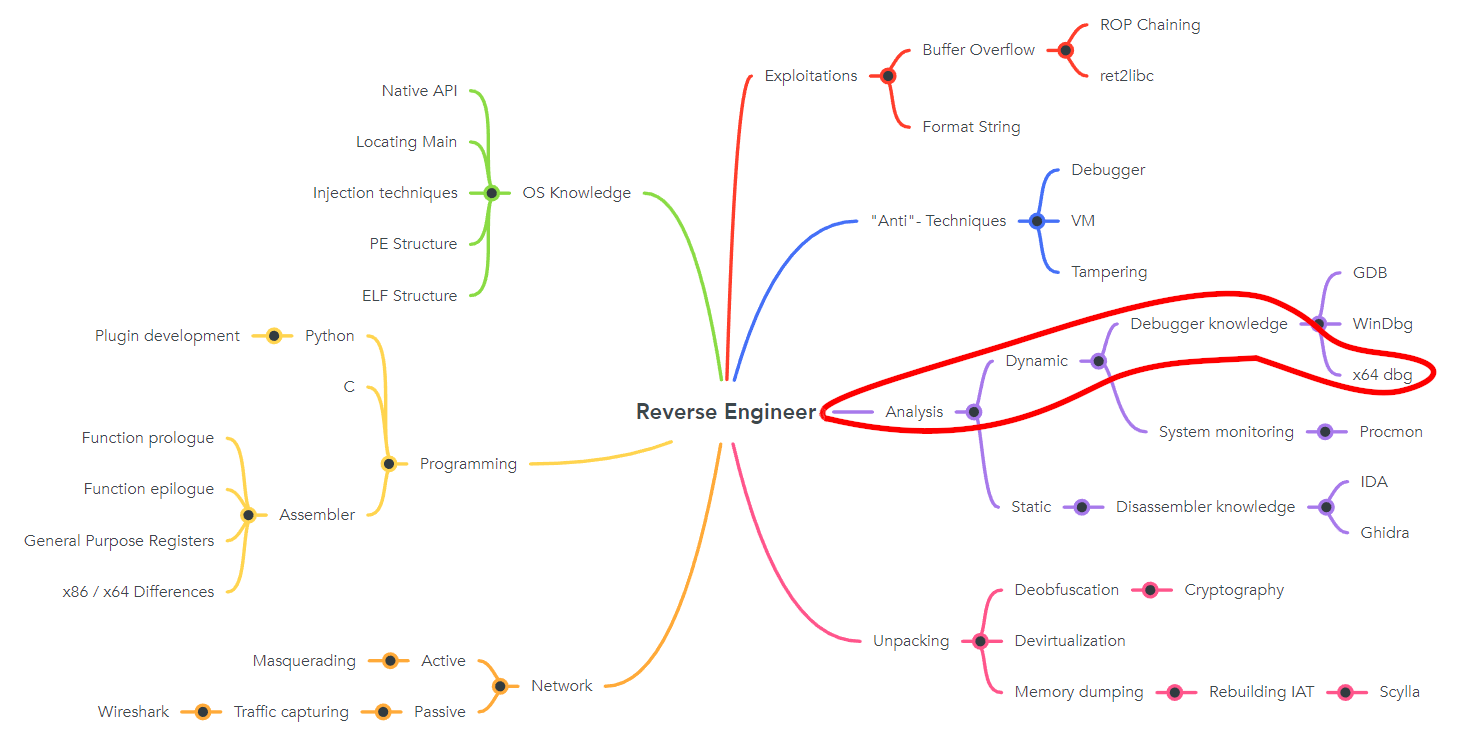
\includegraphics[width=\textwidth]{resources/x64Intro-overview-light.png}
\subsubsection*{Content}
Because most students have probably never touched a debugger on Windows before, this lab will help getting their feet wet with one of the most widely used ones by professionals.
This lab also acts as the basis for the upcoming labs where x64dbg will be used.
\subsubsection*{Choice of Topic}
Students working with Windows should also be given the opportunity to use a debugger. This lab will guide them through the GUI of the program and explain the basic functionality of what is coming up in future labs.
\subsubsection*{Objectives}
\begin{itemize}
    \item Install x64dbg and get a brief overview
    \item Get to know the functionality of x64dbg and be ready to use it on a binary
\end{itemize}
\subsubsection*{Grading}
The introduction labs are not graded since they are only used as a lookup. They have a flag to make sure the students have read the tools.
\pagebreak

\subsection{Tools Introduction: IDA Freeware}
\subsubsection*{Problem Domain}
This lab covers the following aspects of the reverse engineering problem domain created by us: \\
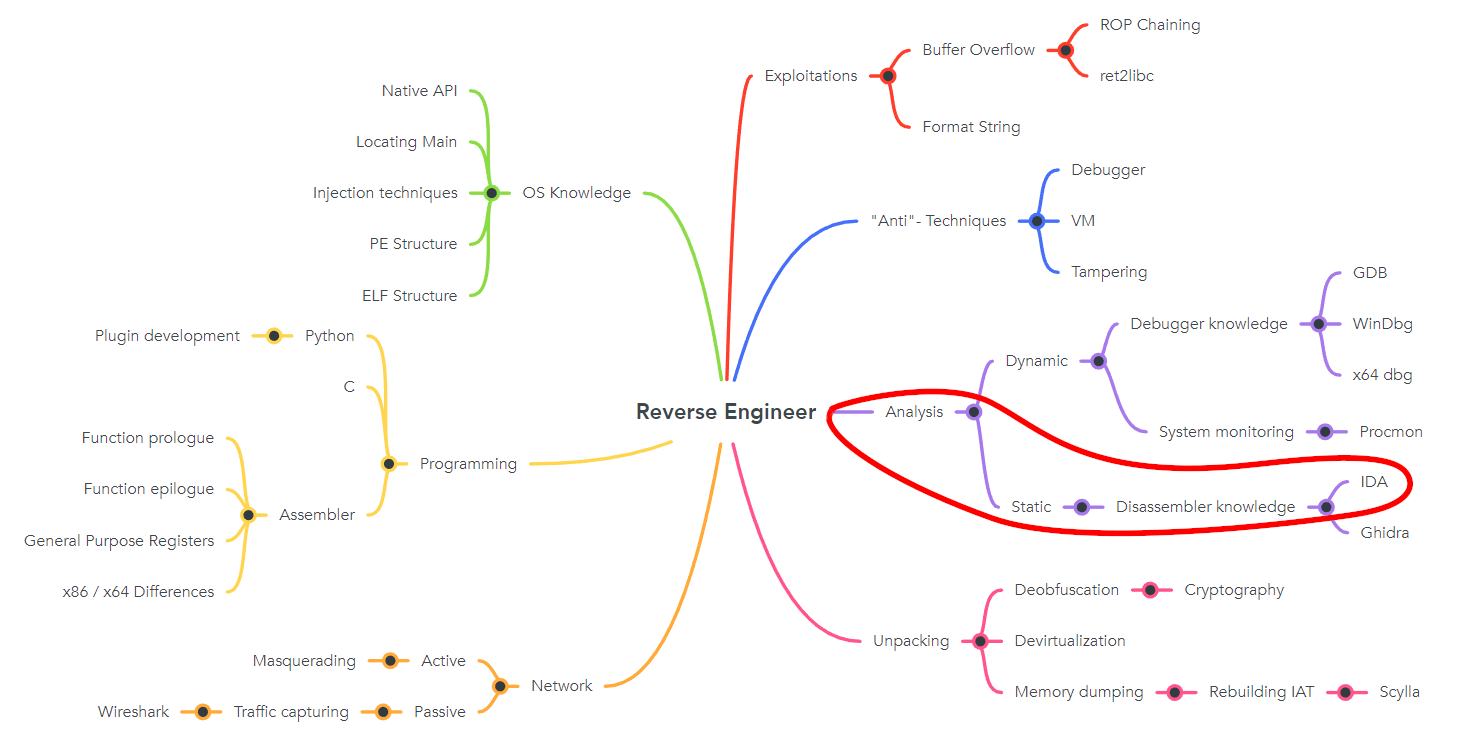
\includegraphics[width=\textwidth]{resources/IDAIntro-overview-light.png}
\subsubsection*{Content}
This introduction explains all the relevant functionalities of IDA and how to install it.
\subsubsection*{Choice of Topic}
Some of the Reverse Engineers most powerful tools are disassemblers. We purposely chose IDA Freeware over Ghidra for the beginning. This prevents the students from just generating pseudo code instead of actually reading and understanding the assembly instructions in later labs. Because of this, the solutions of future labs are presented using IDA Freeware.
\subsubsection*{Objectives}
\begin{itemize}
    \item Install IDA Freeware and get a brief overview
    \item Learn to orient yourself in IDA and get ready to use it on a binary.
\end{itemize}
\subsubsection*{Grading}
The introduction labs are not graded since they are only used as a lookup. They have a flag to make sure the students have read the tools.
\pagebreak
% ------------------------------------------ LABS ------------------------------------------ %

\subsection{Lab 1: Asm-Refresher}
\subsubsection*{Problem Domain}
This lab covers the following aspects of the reverse engineering problem domain created by us: \\
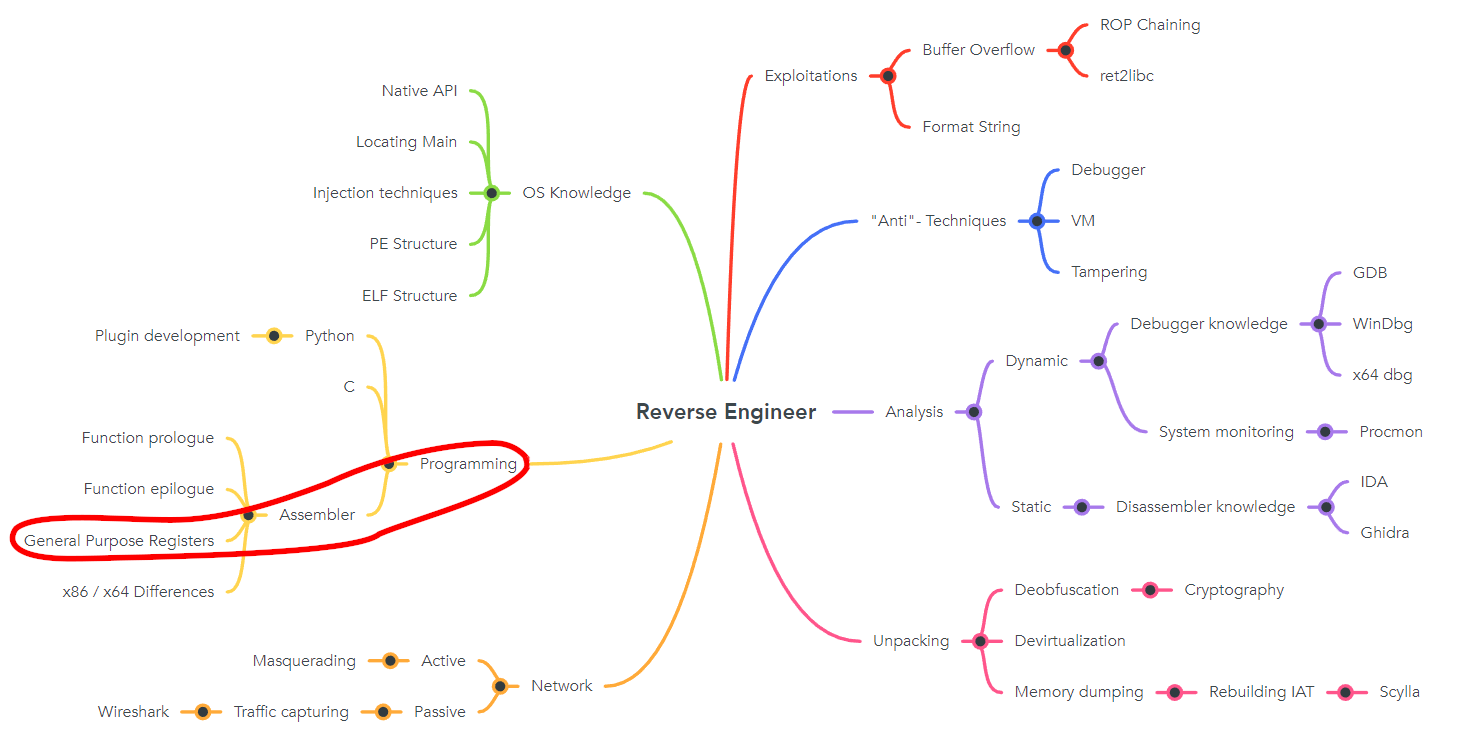
\includegraphics[width=\textwidth]{resources/ASM-overview-light.png}
\subsubsection*{Content}
This lab is designed to be a refresher for those who have not done anything assembly related in a while. It covers the basic assembly instructions, explains the General-Purpose Registers and rounds up with a guide on how to write a "Hello World" program.  
\subsubsection*{Choice of Topic}
A reverse engineer has to understand the basic concepts of assembly. Not only when reading through dissasembled code but also later on when automatic pseudo code generation fails.
\subsubsection*{Objectives}
\begin{itemize}
    \item Refresh knowledge about the general-purpose registers.
    \item Basic understanding of assembly instructions
\end{itemize}
\subsubsection*{Grading}
This lab will not be graded since it is meant to help the students in later labs if they struggle with assembly.
\pagebreak

\subsection{Lab 2: Static Debugging}
\subsubsection*{Problem Domain}
This lab covers the following aspects of the reverse engineering problem domain created by us: \\
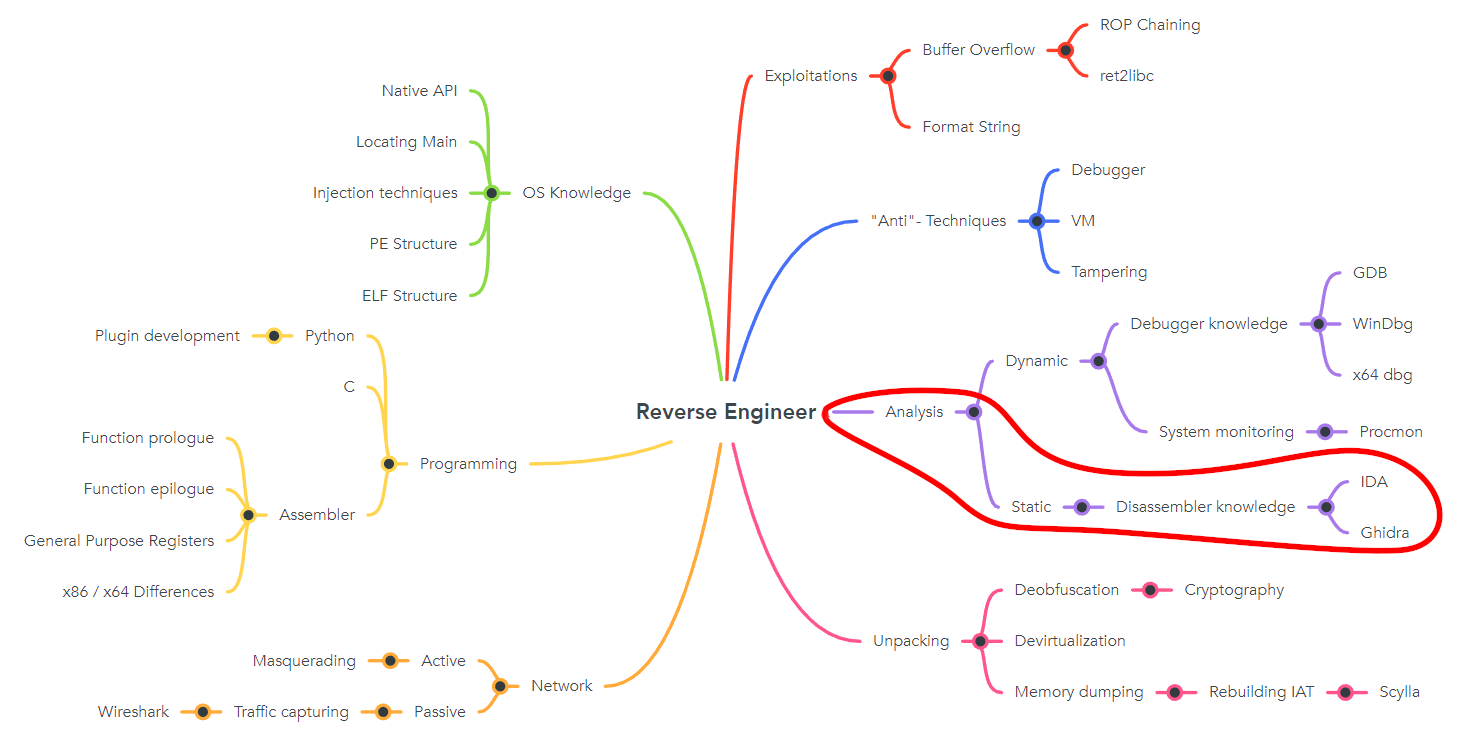
\includegraphics[width=\textwidth]{resources/static-overview-light.png}
\subsubsection*{Content}
In this lab the student will learn how to use IDA Freeware to statically reverse a given binary. The goal is to find the main function in a binary with and one without symbols. \\
This will show the student that seemingly simple things such as finding the main function can be a real problem if you have insufficient knowledge of the inner workings of a binary and the automatic detection of IDA fails.

\subsubsection*{Choice of Topic}
Program execution starts from the main() function which is why it is an important skill of a reverse engineer to find it and start understanding the rest of the binary from there on.
\subsubsection*{Objectives}
\begin{itemize}
    \item Find the main function in a normal binary
    \item Find the main function in a binary with symbols stripped
\end{itemize}
\subsubsection*{Grading}
The student has to inspect the main functions and find a flag in both of them. The final hand-in will be the combined flag.
\pagebreak

\subsection{Lab 3: Dynamic Debugging}
\subsubsection*{Problem Domain}
This lab covers the following aspects of the reverse engineering problem domain created by us: \\
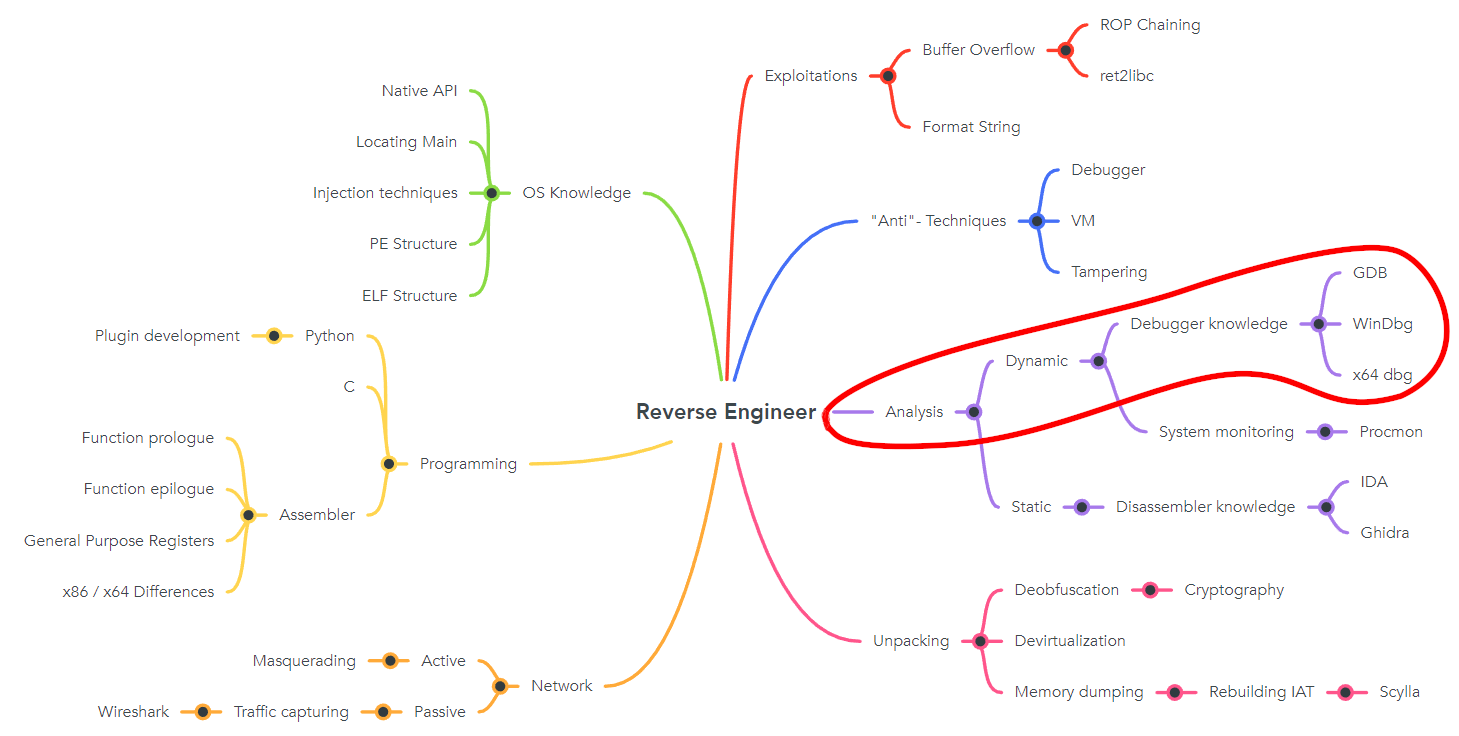
\includegraphics[width=\textwidth]{resources/dynamic-overview-light.png}
\subsubsection*{Content}
In this lab the student will learn how to use GDB and x64dbg to dynamically reverse a given binary. In a first step the lab explains how to dynamically debug the binary given in lab 2 and then, in a second step, the student will be presented with a new binary containing a flag. \\
The goal of this lab is to show the student how this skill is used and then have him do it on his own to solidify the steps he has completed before.
\subsubsection*{Choice of Topic}
Next to static debugging, dynamic debugging is used in a wide range of reverse engineering. Because of this it is important to have a student go through the steps and explain how it is done. 
\subsubsection*{Objectives}
\begin{itemize}
    \item Use GDB to find the flag of the binary
    \item Use x64dbg to find the flag of the binary
    \item Find the flag of a new binary using dynamic debugging
\end{itemize}
\subsubsection*{Grading}
The student has to use the newly aquired skills to find the flag in a new binary using dynamic debugging skills.
\pagebreak

\subsection{Lab 4: First Reversing Attempts}
\subsubsection*{Problem Domain}
This lab covers the following aspects of the reverse engineering problem domain created by us: \\
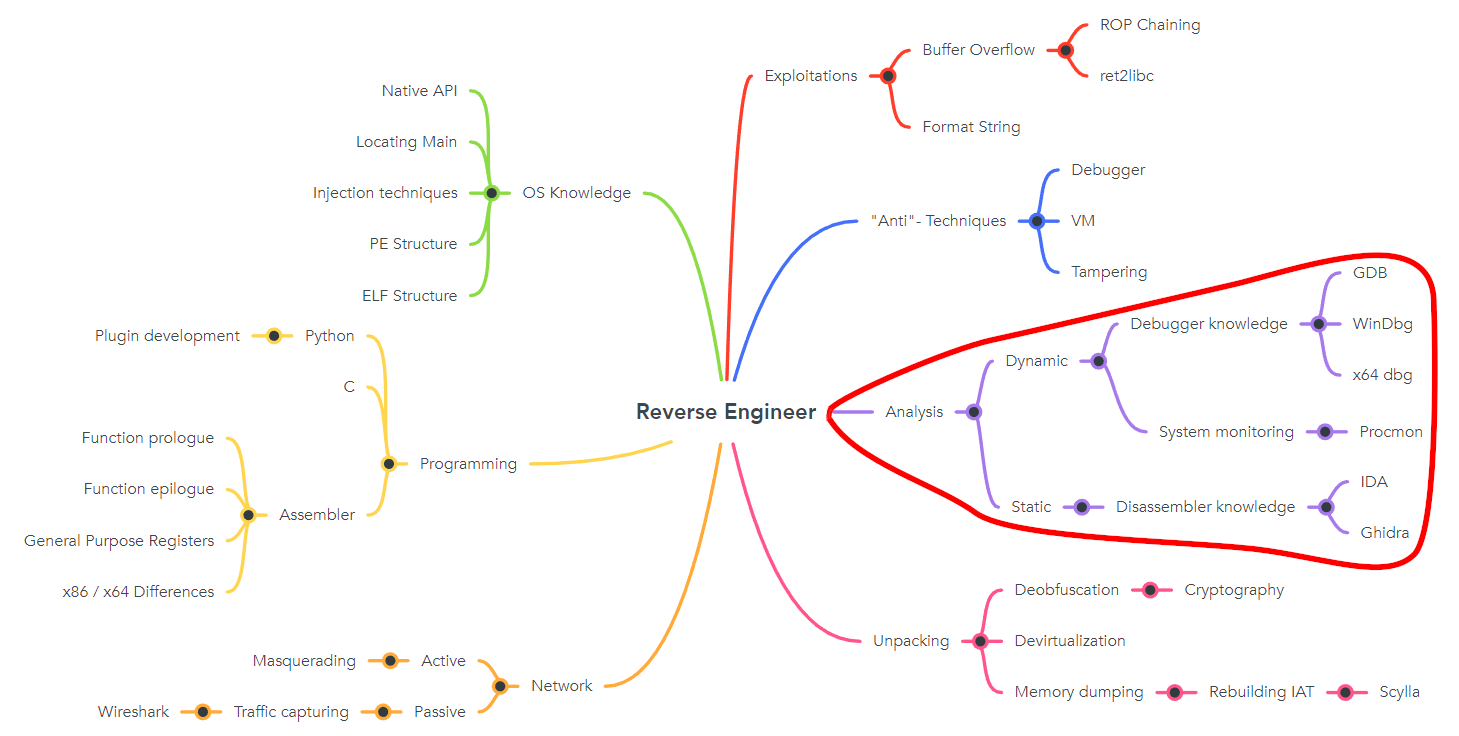
\includegraphics[width=\textwidth]{resources/reattempts-overview-light.png}
\subsubsection*{Content}
In this lab the student will deepen his knowledge of reversing binaries to find out how they work. This challenge contains two binaries having different requirements that have to be met in order for the student to receive the flags.
\subsubsection*{Choice of Topic}
It is important to give the students simple examples where they can play around and learn by doing without providing a step by step guide.
\subsubsection*{Objectives}
\begin{itemize}
    \item Use static or dynamic debugging to find the requirements of the programs
    \item Find out how program arguments are handled in assembly
\end{itemize}
\subsubsection*{Grading}
The student has to solve both binaries to get a flag.
\pagebreak

\subsection{Lab 5: Remote Login}
\subsubsection*{Problem Domain}
This lab covers the following aspects of the reverse engineering problem domain created by us: \\
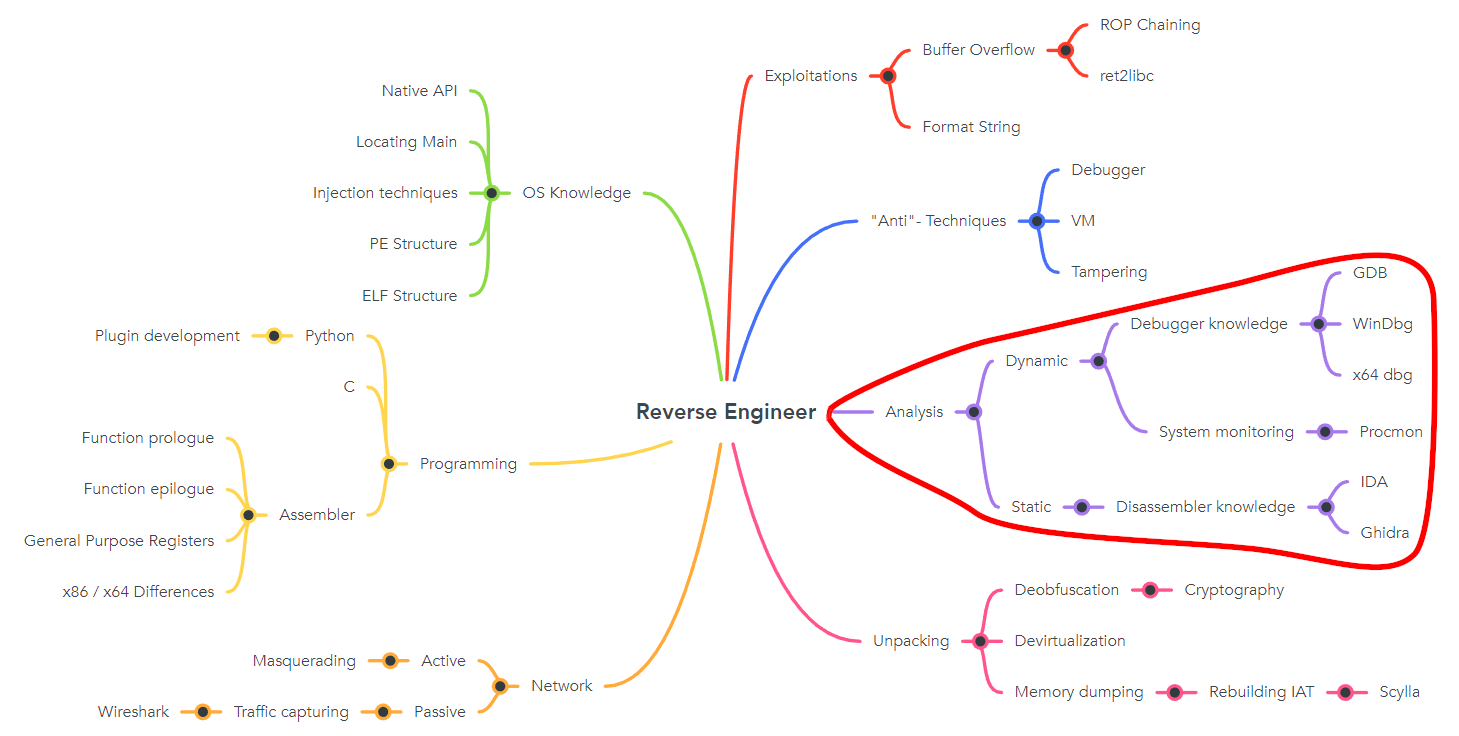
\includegraphics[width=\textwidth]{resources/remotelogin-overview-light.png}
\subsubsection*{Content}
This lab dives deeper into the reverse engineering rabbit hole and introduces a new concept. The student first starts a docker container off a provided resource.
This docker container exposes a webserver and a port where an application runs. The application running on the server can be downloaded from the servers website by the student. \\
The student then has to combine dynamic and static reverse engineering to figure out the password in order to log into the server and expose the flag.
\subsubsection*{Choice of Topic}
Giving the students an idea that reverse engineering can be used to gather information that you can later exploit on a target system.
\subsubsection*{Objectives}
\begin{itemize}
    \item Learn to use the tools you got introduced to
    \item Apply basics of dynamic and static debugging
    \item Use gatherd knowledge to exploit remote target
\end{itemize}
\subsubsection*{Grading}
The student has to find out the flag and submit a small writeup to answer the security questions provided.
\pagebreak

\subsection{Lab 6: Pwntools - Introduction}
\subsubsection*{Problem Domain}
This lab covers the following aspects of the reverse engineering problem domain created by us: \\
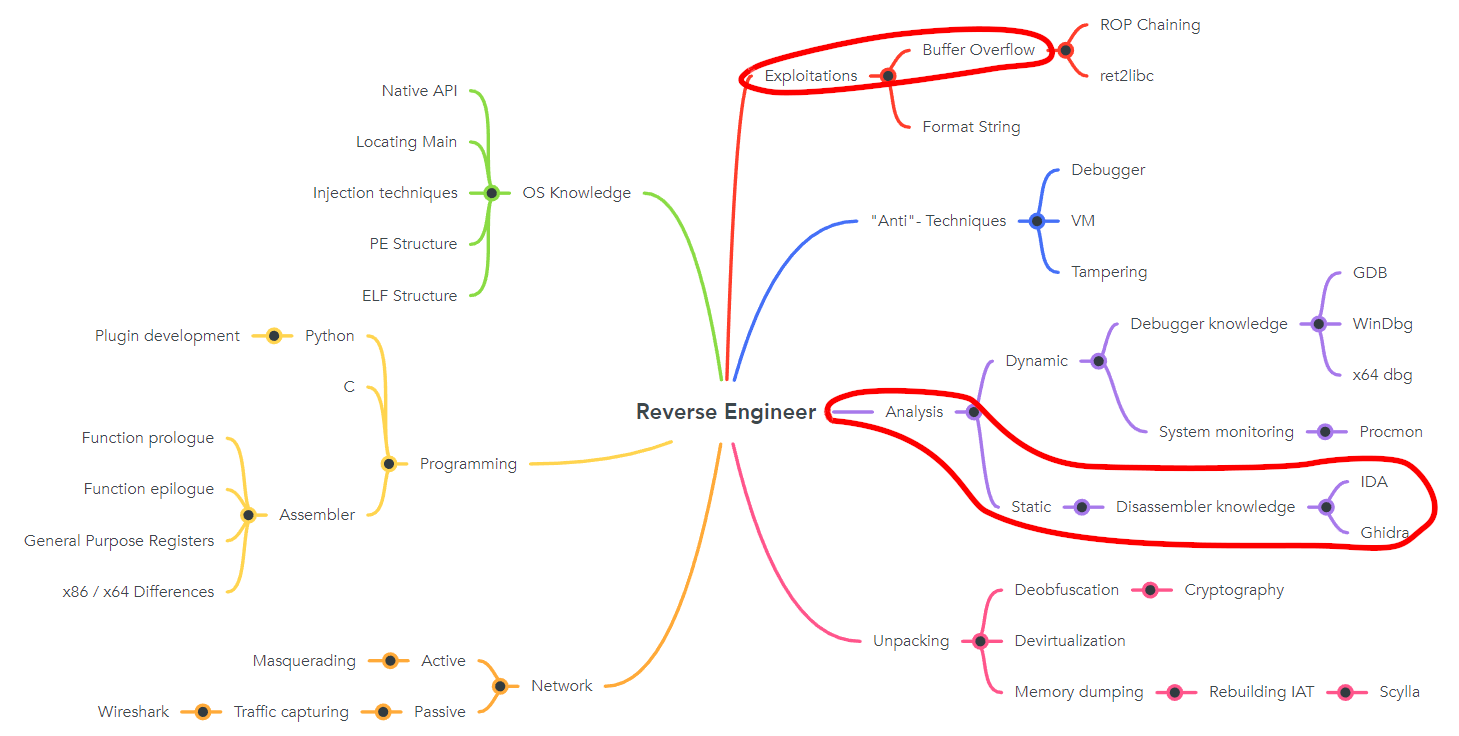
\includegraphics[width=\textwidth]{resources/pwntools-overview-light.png}
\subsubsection*{Content}
In this lab the student has a first introduction into the pwntool module of python. The student first has to start a docker conatiner from the provided resource. This docker exposes both a webserver and a port where the application is running on. The student then downloads the compiled application to analyze it and search for a weakness to exploit. This weakness can then be exploited through the use of pwntools. Since this is a first introduction, the whole process of creating the script is guided as a walkthrough.
\subsubsection*{Choice of Topic}
Pwntools is an important module to learn for exploiting. Reverse engineering in general is widely used to find vulnerabilities to exploit, which means it is important for a student to not only know how to find the weakness but also how to exploit it.
\subsubsection*{Objectives}
\begin{itemize}
    \item Use acquired skills to find vulnerability in binary
    \item Create a pwntools script to exploit that vulnerabilty
\end{itemize}
\subsubsection*{Grading}
The grading is done by sending in the printed out flag when the script is run on the exposed port and a writeup answering the provided security questions.
\pagebreak

\subsection{Lab 7: Crypto Lab - AES ECB}
\subsubsection*{Problem Domain}
This lab covers the following aspects of the reverse engineering problem domain created by us: \\
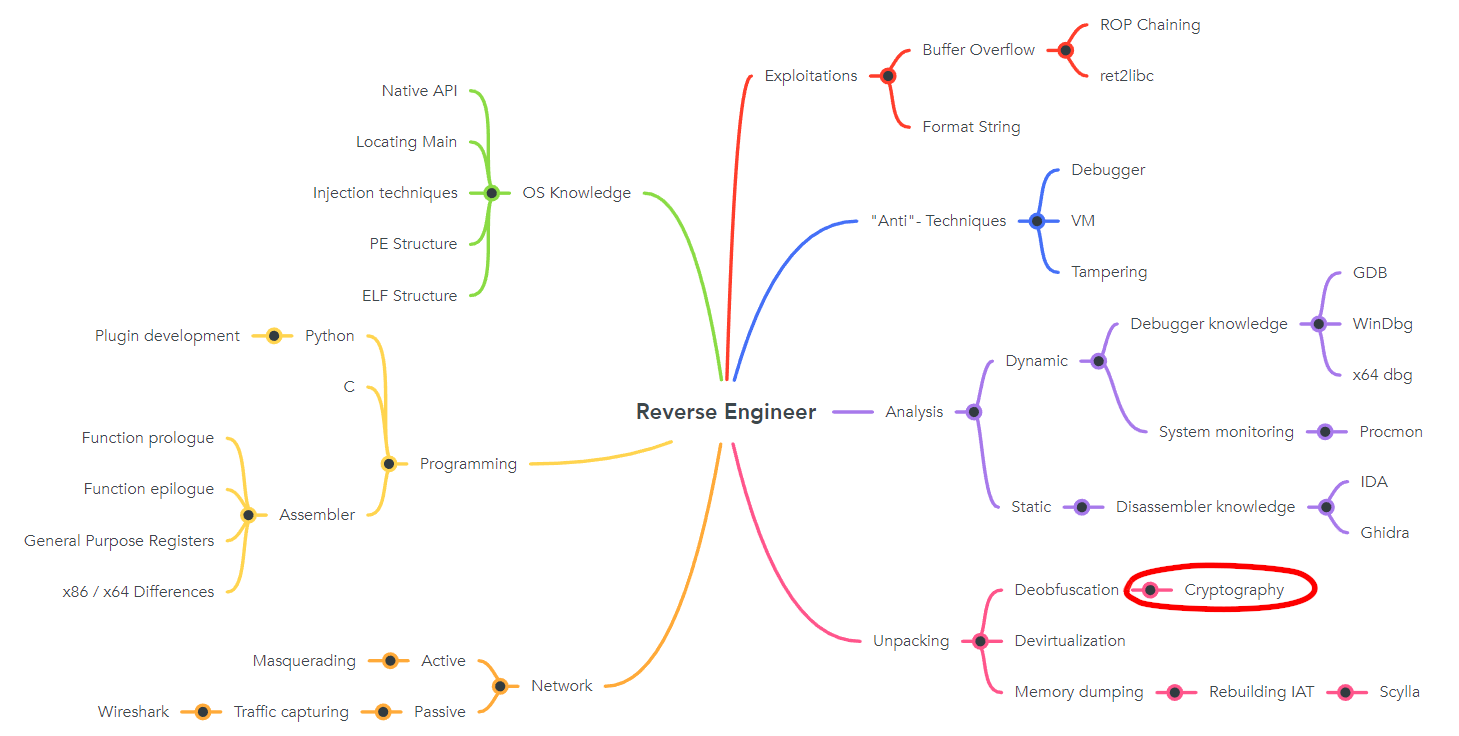
\includegraphics[width=\textwidth]{resources/aes-overview-light.png}
\subsubsection*{Content}
The student is presented a docker container which runs a webserver and exposes a port on which the script for the student to crack is running. The student first inspects and analyzes the script itself and then follows a walkthrough on how to write a simple script which exploits a common vulnerability in AES ECB mode. 
\subsubsection*{Choice of Topic}
Encryption is a widely used form of obfuscation. Because of this it is important as a cyber security student to be informed about certain weaknesses these ciphers have and how to exploit them if needed. 
\subsubsection*{Objectives}
\begin{itemize}
    \item Find out how the script works
    \item Find patterns to exploit
    \item Create a pwntools script to crack the encryption
\end{itemize}
\subsubsection*{Grading}
The grading is done by sending in the printed out flag when the script is run on the exposed port in combination with a writeup answering the provided security questions.
\pagebreak

\subsection{Lab 8: Patching Lab}
\subsubsection*{Problem Domain}
This lab covers the following aspects of the reverse engineering problem domain created by us: \\
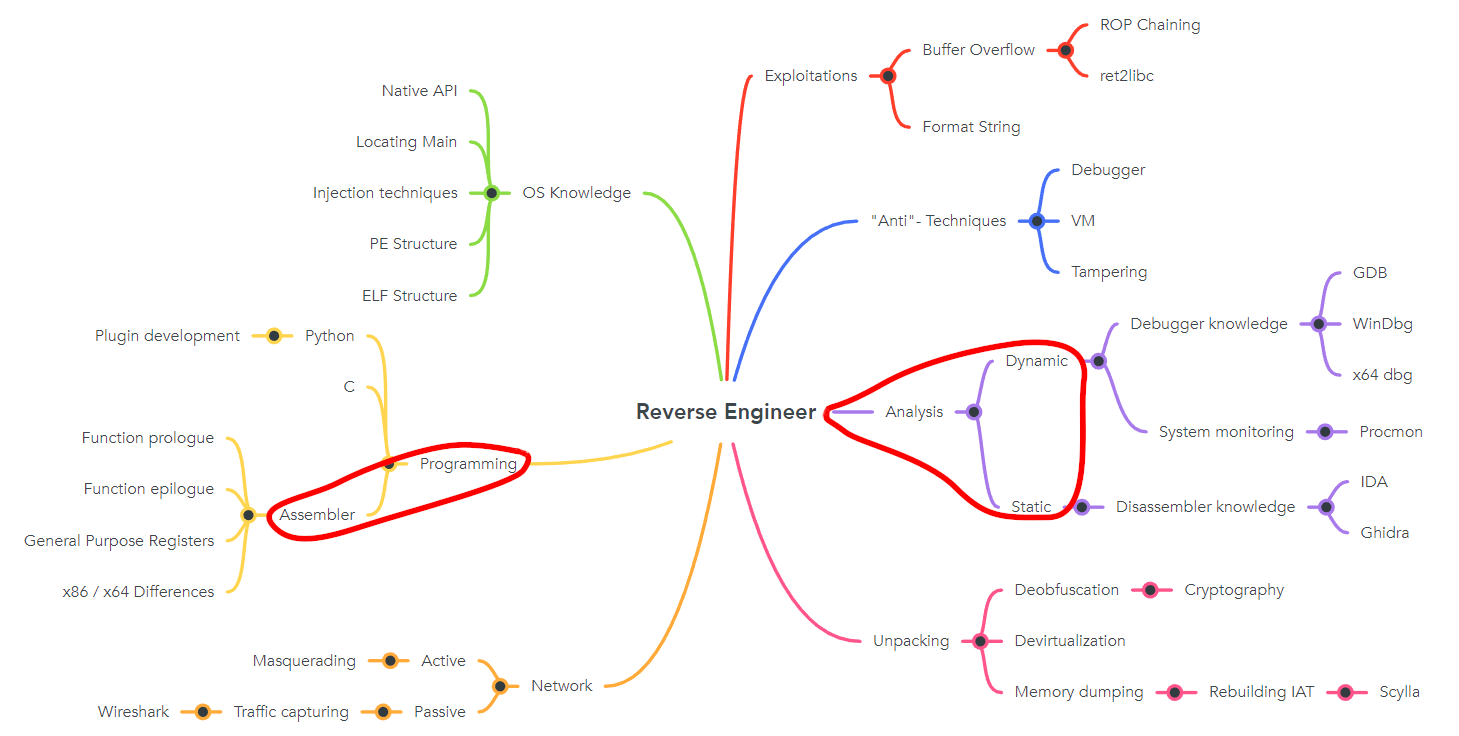
\includegraphics[width=\textwidth]{resources/patching-overview-light.png}
\subsubsection*{Content}
The student is presented a binary which does not operate correctly. The student is tasked to find the location to patch and fix it. In order to check the patch generated by the user, the provided docker container starts up a webserver where the student can upload the patch file. The webserver then tries to apply the patch to a local copy of the binary and checks if the bug is fixed. If fixed, the webserver shows the flag to the student. If not fixed, the student has the possibility to reset the binary and try again.

\subsubsection*{Choice of Topic}
Reverse engineering also comes in handy when encountering bugs in software where the source code is unreachable. Therefore it is important to locate found bugs in an executable and know how to apply patches.
\subsubsection*{Objectives}
\begin{itemize}
    \item Find the mistake of the binary
    \item Change the ASM code
    \item Patch the file
\end{itemize}
\subsubsection*{Grading}
The grading will be done via a writeup and a flag.
\pagebreak
